\section{Background}\label{sec:background}

\begin{figure}[t!]
\centering
\includegraphics[width=0.5\textwidth]{figs/RRC_State_Diagram.pdf}
\ncaption{Possible 3G and 4G State Machines as Specified by 3GPP.} 
\label{fig:statemachine}
%\begin{center}
%\includegraphics[width=0.5\textwidth]{figs/4g_rrc.png}
%\end{center}
%\ncaption{4G LTE state machine based on our inference methodology}
%\label{fig:4G_statemachine}
\vspace{0.5em}
\end{figure}

\begin{figure}[t!]
\centering
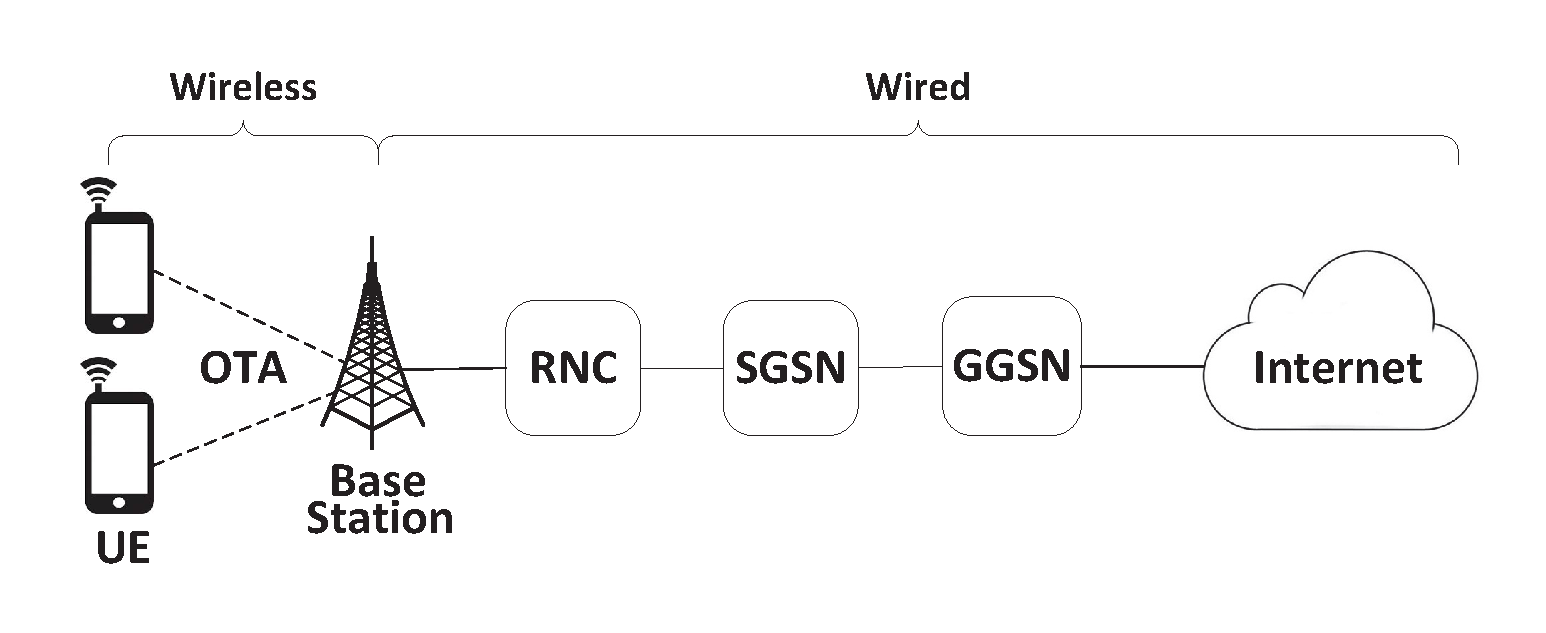
\includegraphics[width=0.5\textwidth]{figs/cellular_network_topology.eps}
\ncaption{The general cellular network architecture}
\label{fig:cell.topology}
\end{figure}

As illustrated in Figure~\ref{fig:cell.topology}, in both 3G UMTS~\cite{3gpp.3G} and 4G LTE networks~\cite{3gpp.lte}, data is transmitted from \textit{user equipment} (UE), i.e. mobile devices,  to the base station (Node B in UMTS, eNB in LTE), then to the \textit{Serving GPRS support node} (SGSN) and \textit{Gateway GPRS support node} (GGSN), and ultimately to the server~\cite{umts_book}. The link between the UE and the base station is known as the \textit{over-the-air} (OTA) link, and it is the only wireless link in the network topology. The rest of the links from the base station to the internet are all wired.

Mobile cellular networks use the Radio Resource Control (RRC) protocol to allocate resources to mobile devices.  Handsets transition between different RRC states, which vary in power consumption and bandwidth, and an individual RRC state machine is maintained for each handset.  Transitions between different states occur due to traffic patterns between the device and base station. In general, more traffic will cause a higher-power and higher-bandwidth state to be entered.  The RRC protocol for these network types has been defined by 3GPP~\cite{spec-3G-RRC, spec-LTE-RRC}.

Different carriers implement RRC state machines differently, with state transitions and different associated timers varying between carriers.  However, for 2G, 3G and 4G LTE, there are a fixed set of possible states defined. We give a brief overview below; a more detailed overview can be found in previous work~\cite{3g_rrc, 4g_rrc}.

\begin{table*}[th!]\small
\begin{tabularx}{\textwidth}{ | c | c | X | }
\hline
\textbf{Category} & \textbf{Label} & \textbf{Description} \\
\hline
\hline
%\multicolumn{2}{|c|}{\textbf{3G UMTS - Specification}} \\
%\hline
%\multirow{3}{*}{\textbf{\vbox{3G UMTS - Specification}}} & DCH & high-power, high-bandwidth\\ \cline{2-3}
\multirow{3}{*}{\textbf{3G UMTS - RRC States in Specification}} & DCH & High-power, high-bandwidth\\ \cline{2-3}
& FACH & Low-power, low-bandwidth\\ \cline{2-3}
& PCH & No transmission possible\\
\hline
%\multicolumn{2}{|c|}{\textbf{3G UMTS - Observed Phenomena}} \\
%\hline
%\multirow{7}{*}{\textbf{\vbox{3G UMTS - Observed Phenomena}}} & FACH TRANSITION & period of high latency when transitioning from DCH to FACH\\ \cline{2-3}
\multirow{5}{*}{\textbf{3G UMTS - Newly-detected Transient States}}
& FACH INIT & Initial FACH state interval with \textit{frequent} link layer retransmission\\ \cline{2-3}
& FACH PROMOTE & State transition interval from FACH to DCH with signalling overhead\\ \cline{2-3}
& FACH STABLE & Time interval in between FACH INIT and FACH PROMOTE\\ \cline{2-3}
& PCH INIT & Initial PCH state interval with \textit{few} link layer retransmission\\ \cline{2-3}
& PCH PROMOTE & State transition interval from PCH to FACH with signalling overhead\\ \cline{2-3}

\hline
\multirow{1}{*}{\textbf{3G UMTS - UDP-Layer Observed Behavior}} & FACH TRANSITION & Period of high latency when transitioning from DCH to FACH\\
\hline
\hline
%\multicolumn{2}{|c|}{\textbf{4G LTE - Specification}} \\
%\hline
%\multirow{2}{*}{\textbf{\vbox{4G LTE - Specification}}} & RRC CONNECTED & high-power, high-bandwidth \\ \cline{2-3}
\multirow{2}{*}{\textbf{4G LTE - RRC States in Specification}} & RRC CONNECTED & High-power, high-bandwidth \\ \cline{2-3}
& RRC IDLE & No transmission possible \\
\hline
%\multicolumn{2}{|c|}{\textbf{4G LTE - Observed Phenomena}} \\
\hline
%\multirow{1}{*}{\textbf{\vbox{4G LTE - Observed Phenomena}}} & FACH TRANSITION & period of high latency when transitioning from DCH to FACH \\
\multirow{1}{*}{\textbf{4G LTE - UDP-Layer Observed Behavior}} & LTE TRANSITION & Period of high latency when demoting from RRC CONNECTED to RRC IDLE\\
\hline
\hline
%\multicolumn{2}{|c|}{\textbf{QxDM Related}} \\ 
%\hline
\multirow{3}{*}{\textbf{QxDM Related}} & RLC retx ratio & $\frac{\textit{\# of Retx PDUs in \textbf{T}}}{\textit{Total \# of PDUs in \textbf{T}}}$ , where \textit{\textbf{T}} is a range of time \\ \cline{2-3}
& UDP loss ratio & $\frac{\textit{\# of UDP packets \textbf{NOT} received by receiver in \textbf{T}}}{\textit{Total \# of UDP packets that the sender transmitted in \textbf{T}}}$ , where \textit{\textbf{T}} is a range of time \\ \cline{2-3}
& Inter-packet interval & Time between when a test packet is sent and when a high-power state is induced, for the purpose of measuring timers. \\ \cline{2-3}
\hline
\end{tabularx}
\ncaption{Summary of key terminology used.} % Terminology should not be plural, a terminology is a set of terms and we have only one set of terms. https://en.wiktionary.org/wiki/terminology
\label{tab:terminology}
\end{table*}

For 3G UMTS~\cite{spec-3G-RRC}, there are three main states:  DCH, which is high-power and high-bandwidth, FACH, which is low power and low bandwidth, and PCH, where no transmission is possible. If a higher-bandwidth state is needed, there is a promotion delay. Some carriers may always go directly from PCH to DCH. An example RRC state machine can be seen at the top of Figure~\ref{fig:statemachine}. These terms are summarized in Table~\ref{tab:terminology}.
%As a further complication, UMTS supports \emph{fast dormancy}. The user device is able to proactively request to transition to IDLE to reduce the tail time after a data transmission where the device is a higher-power state than necessary~\cite{fast_dormancy, spec-3G-RRC}.

For 4G~\cite{spec-LTE-RRC}, the state machine is more complicated, and is summarized in the bottom half of Figure~\ref{fig:statemachine}.  We are concerned mainly with transitions between RRC\_{}CONNECTED, a higher-power state, and RRC\_{}IDLE, a lower-power state where no data is transmitted. The other states have timers on the orders of tens or hundreds of milliseconds are are not practical to measure on end-user devices, as tools such as a power monitor are required.

%There are two main states: RRC\_{}CONNECTED, a higher-power state, and RRC\_{}IDLE, a lower-power state.  RRC\_{}IDLE periodically wakes up to determine if it needs to promote to a higher-power state.  This is known as Discontinuous Reception or DRX.  We would like to infer the timer to fall back to RRC\_{}IDLE, as well as the time between ON segments in RRC\_IDLE and the length of those segments.

%For RRC\_CONNECTED, there are several additional substates.  After a data transfer, the device remains in Continuous Reception for some time, before transitioning to Short DRX.  Similarly to DRC for RRC\_IDLE, the device sleeps for a short period of time, waking up periodically to check if there is data, but the sleep time is much shorter.  There is another timer to transition to Long DRX, which has a longer sleep timer than Short DRX, but still a much shorter one than in RRC\_IDLE. Additionally, the ON timers for the three DRX states can vary~\cite{spec-LTE-RRC}.

Determining when to fall back to a low power state can have a substantial impact on performance, as can the state transitions supported.  If demotion happens early, then there will be additional promotion delays, resulting in decreased user performance.  If it happens late, then an unnecessary amount of power will be consumed. For this reason, we wish to understand how carriers implement RRC state machines in practice.

Furthermore, we found that network traffic often does not follow the ideal pattern expected by the RRC specification, another major motivation for understanding RRC state behavior in the real world.  This occurs in particular during state transitions, where certain transitions on certain devices can lead to substantial delays, so we define terms to refer to these phenomena which we will use throughout the paper. There is often a significant additional promotion delay immediately after a state demotion, especially a demotion from DCH to FACH.  We refer to this phenomenon as \emph{FACH\_{}TRANSITION} when it occurs immediately before FACH, and \emph{LTE\_{}TRANSITION} when it occurs in LTE. 

To understand the root cause of this unexpected behavior, we observed behavior at the RLC layer.  We break down the behavior in each state at the RLC layer into several smaller \emph{transient states} as shown in Figure~\ref{fig:qxdm.rrc.state}.  

% XXX I rewrote this paragraph.
We define the FACH\_{}PROMOTE and PCH\_{}PROMOTE transient states based on behavior observed at the RRC layer. These states end when the new RRC state is logged by QxDM and start when the previous IP data packet was sent.  We describe the experiments to determine when this period occurs in~\ref{sec:exp.setup}.  The FACH\_{}INIT transient state corresponds to a period of high RLC retransmissions determined experimentally from the QxDM traces.  The period of FACH not covered by FACH\_{}PROMOTE and FACH\_{}INIT we define to be FACH\_{}STABLE.  There is no corresponding PCH\_{}STABLE state as no data is sent in PCH.  Therefore, the PCH\_{}INIT transient state refers to the period of time in PCH during our tests where the device is not in PCH\_{}PROMOTE.  We determined that the FACH\_{}TRANSITION delays occur primarily due to losses in the transition states FACH\_{}INIT and FACH\_{}PROMOTE.

%Both the FACH\_{}PROMOTE and PCH\_{}PROMOTE transition states are determined by the average time interval between the last IP data packet log timestamp to the next RRC state log timestamp from the local QxDM experiments that will be defined in ~\ref{sec:exp.setup}. The FACH\_{}INIT substate is where the high RLC retransmission occurs. We determine the average time interval value where the substantial high RLC retransmission from those QxDM experiments as well. We exclude the whole FACH state period by the FACH\_{}PROMOTE and FACH\_{}INIT to get FACH\_{}STABLE substate. The PCH\_{}STABLE substate doesn't exist since the device cannot stay in PCH during the PCH to FACH promotion. So we determine the PCH\_{}INIT substate period by subtracting PCH\_{}PROMOTE substate interval from the PCH state interval.

\begin{figure}[t!]
\centering
\includegraphics[width=0.5\textwidth]{figs/qxdm_rrc_state_no_pch_stable.eps}
\vspace{-2.5ex}
\ncaption{RRC transient state definitions from observed RLC-layer behavior during state promotions. We examine these individually through QxDM to investigate root causes of latency.} 
\label{fig:qxdm.rrc.state}
\vspace{-1.5ex}
\end{figure}

%We call the period of time immediately after a promotion from DCH to FACH \emph{FACH\_{}INIT}, and the period of time where FACH promotes to DCH \emph{FACH\_{}PROMOTE}.  FACH\_{}TRANSITION occurs where FACH\_{}INIT is immediately followed by FACH\_{}PROMOTE; FACH\_{}TRANSITION refers to a type of behavior observed at the UDP layer and not to RLC-level behavior.  Similarily, PCH is divided into \emph{PCH\_{}INIT} and \emph{PCH\_{}DEMOTE}.

%\mycomment{these terminology on INIT, PROMOTE, and DEMOTE are not quite clear, maybe explain in terms of signaling required:  Does INIT mean that there are still signaling occurring?}
